\section{Architecture}\label{sec:Architecture}




% Describe the data processing pipeline here. 


% 1. Get the raw data and remove the ground (LiDAR data clean up)
% 2. Segment data and sent it to classifier 
% 3. Classification with Neural Network. 


Figure \ref{fig:dataPipeline} depicts  

\begin{figure*}[h!]
 \begin{center}
   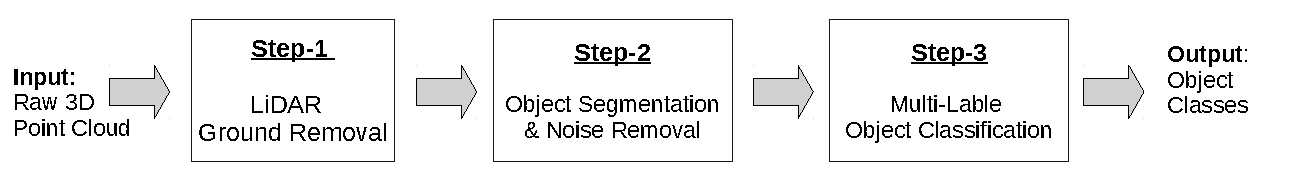
\includegraphics[width=0.9\textwidth]{./images/DataProcessingPipleline.pdf}
   \caption{An Overview of our Data Processing Architecture}
   \label{fig:dataPipeline}
 \end{center}
\end{figure*}





Describe \ldots. 

Different forms of data processing architectures that we have implemented and tested . 

\begin{enumerate}
  \item Different methods for removing noise from raw data (data preprocessing). 
  \item Projecting 3D data into 2D data using 3 different projection methods 
  \item CNN  (with and without maxpool) + fully-connected + dropout + fully-connected+softmax
  \item CNN with different number of hidden layers. 

\end{enumerate}



% KIA
% We need another image to describe the CNN architecture. 
% Add two images about it. 



